%main for analyse

\part{System Analysis}
\label{system_analysis}

\chapter{Description of Water Supply Systems}
\label{description_of_water_supply_systems}

 \emph{This chapter gives a general overview of hydraulic systems and an introduction to the WSS in Randers. The basic topology and structures of water supply networks are explained. }

\section{Hydraulic system overview}
\label{hydraulic_system_overview}

WSSs are designed to deliver water to consumers in terms of sufficient pressure and appropriate chemical composition. Distribution systems as such are typically transport water from one geographical place to another. In practice, there are different methods existing to achieve this water transport. One example is to make use of natural advantages such as the water stored in mountains, and therefore use the potential energy to provide pressure in the network. Good examples are countries like Norway and Sweden where the advantages of the landscape can be exploited. However, in this project the origin of the water is considered as groundwater, considering that in Denmark all reservoirs in the network are tapping water from the ground. After tapping the water, it goes through a cleaning process at the waterwork and afterwards the pure water is pumped into the network \cite{prahata}. In WSSs, pumps and valves are the elements that enable the delivery of water to the consumers or to elevated reservoirs, storing water for later use. Such a network is illustrated in the figure below: 

%illustration of WSS
\begin{figure}[H]
\centering
\includegraphics[width=0.35\textwidth]{report/pictures/missingfigure}
\caption{Illustration of a WSS.}
\label{fig:WSS_example}
\end{figure}

The delivered water needs to fulfil a certain pressure criteria in order to reach consumers at higher levels. For example, in some cases the pressure has to be high enough to make it to the fourth floor of a building and still provide appropriate pressure in the water taps. In such cases, generally booster pumps are placed in the area, helping to supply pressure. Too large pressure values however  increase water losses due to pipe waste \cite{walski2003advanced}.

Another criteria is that the flows through particular pipes need to stay within acceptable limits. A low flow rate can lead to water quality problems due to the undesirable microorganisms in the water and due to the metal and salt accumulation on the wall of the pipes \cite{walski2003advanced}. 

As can be seen in \figref{fig:WSS_example}, typically WSSs consist of pipe, valve, reservoir, elevated reservoir(tank) and pump components. The common property of these components is that they are all two-terminal components, therefore they can be characterized by the dynamic relationship between the pressure drop across the two endpoints and the flow through the elements \cite{master_aau}. 

\subsection{Pipe system}
\label{pipe_system}

Pipes are the most common components of WSSs since they are used for carrying pressurized water. They serve as a connection between components. The network can be separated into different subsections, concerning the physical size and purpose of the pipes. Water supply networks consist of transmission mains, arterial mains, distribution mains and service lines as shown in the example below: 

%illustration of pipe topology / loop configuration
\begin{figure}[H]
\centering
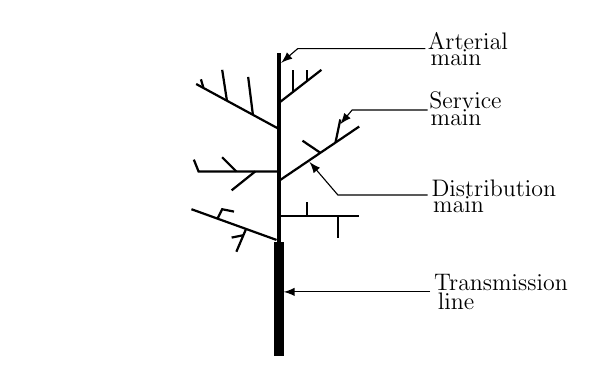
\begin{tikzpicture}[scale=0.6,transform shape]

\fill [black] (0.1,0.1) rectangle (0.3,2.5);
\fill [black] (0.15,6.5) rectangle (0.25,2.5);

\draw [thick](0.15,2.55) -- (-1.65,3.2);
\draw [thick](-0.5,2.77) -- (-0.7,2.3);
\draw [thick](-0.55,2.65) -- (-0.8,2.6);
\draw [thick](-1.1,3) -- (-1,3.2) -- (-0.75,3.15);
\draw [thick](0.2,3.05) -- (1.9,3.05);
\draw [thick](0.8,3.05) -- (0.8,3.35);
\draw [thick](1.45,3.05) -- (1.45,2.6);
\draw [thick](0.2,4) -- (-1.5,4) -- (-1.6,4.25);
\draw [thick](-0.3,4) node (v1) {} -- (-0.8,3.6);
\draw [thick](v1);
\draw [thick](-0.7,4) -- (-1,4.3);
\draw [thick](0.2,3.8) -- (1.9,4.95);
\draw [thick](1.4,4.62) -- (1.5,5.1);
\draw [thick](1.07,4.4) -- (0.7,4.65);
\draw [thick](0.2,4.9) -- (-1.55,5.85);
\draw [thick](-0.35,5.2) -- (-0.45,6);
\draw [thick](-0.9,5.5) -- (-1,6.15);
\draw [thick](-1.4,5.78) -- (-1.45,5.95);
\draw [thick](0.2,5.45) -- (1.1,6.15);
\draw [thick](0.8,5.92) -- (0.8,6.15);
\draw [thick](0.5,5.69) -- (0.5,6.15);
%\draw [-latex](3.4,1.45) -- (0.3,1.85);
\node at (4.9,1.65) {\Large Transmission};
\node at (3.95,1.25) {\Large line};
%\draw [-latex](3.35,3.4) -- (0.6,4.05);
\node at (4.75,3.65) {\Large Distribution};
\node at (4,3.3) {\Large main};
\node at (4.15,5.5) {\Large Service};
\node at (3.95,5.15) {\Large main};
\node at (4.2,6.75) {\Large Arterial};
\node at (3.95,6.4) {\Large main};
%\draw [-latex](3.25,5.25) -- (1.5,5);
%\draw [-latex](3.2,6.55) -- (0.25,6.4);
\node at (-5,3.6) {         };
\draw [-latex](3.3,6.6) -- (0.6,6.6) -- (0.25,6.3);
\draw [-latex](3.35,5.3) -- (1.75,5.3) -- (1.5,5);
\draw [-latex](3.35,3.5) -- (1.45,3.5) -- (0.85,4.2);
\draw [-latex](3.4,1.45) -- (0.3,1.45);
\end{tikzpicture} 
\caption{Illustration of pipe mains. Tree configuration.}
\label{fig:pipemain_example}
\end{figure}

Transmission mains deliver large amounts of water over long distances. Arterial and distribution mains provide intermediate steps towards delivering water to the end-users. Service lines transmit the water from the distribution mains straight to the end-users \cite{grigg2012water}.

The transmission and distribution network can have a topology that is called a loop or a tree structure. \figref{fig:pipemain_example} shows an example for a tree configuration. This type of configuration is most frequently found in rural areas \cite{mays}. Typically the network has only one path for water to reach the end-users. Common problems with this configuration is that on the outer parts of the system lower pressures can be experienced due to the pressure losses from long flow paths. The flow dynamics within this kind of systems therefore consist of large flows closer to the source that turns into smaller flows on the outer parts of the system. Main disadvantage of a purely tree structure system is that due to maintenance or momentary breakdowns, the system suffers disruption of service \cite{mays}. 

Loop networks have a configuration as shown in \figref{fig:loop_configuration}. 

%illustration of loop configuration
\begin{figure}[H]
\centering
\includegraphics[width=0.35\textwidth]{report/pictures/missingfigure}
\caption{Loop configuration.}
\label{fig:loop_configuration}
\end{figure}

Loop networks are usually composed of smaller loops which made up of smaller distribution mains, and larger loops that are connected to arterial or transmission mains. Elevated reservoirs are typically placed in the centre of the system due to pressure losses resulting from flows through the loop network \cite{council2007drinking}. In the presence of the larger loops, they may be used to feed an internal distribution grid or a distribution grid attached to the outer part of the loop. Loop configurations are generally associated with larger suburban and city distribution systems such as the WSS in Randers\cite{council2007drinking}. 

\subsection{Elevated reservoirs}
\label{elevated_reservoirs}

Elevated reservoirs are typically placed in the system to use them as buffers and level out the pressure and flow demand differences. When the demand is high, the waterworks might not be able to provide the sufficient amount of water in the network. In these cases, the elevated reservoir supplies the remaining demand to the network. When the user consumption decreases, the system can be controlled such that the tank is being refilled to provide the required demand for the next peak. Having such an elevated reservoir in the network, the system becomes more independent of the pump stations, as the refilled tank can itself maintain the desired pressure and flow for a limited time. 

Due to the elevation of the tank, when it is filled up, the pumping stations need to provide a pressure higher than the pressure in the water tank. Therefore when the tank is being emptied, the pumping stations can reduce the amount of pressure they provide to the system, since the pressure from the elevated reservoir becomes dominant. This is due to that the dynamics of systems with large storages come primarily from the pressure of the tank(cite). This is due to the height change of the tank being very slow because of the large diameter of the tank. For these considerations, the effect of these elevated reservoirs has to be taken into account while modelling the system. 

\subsection{Pumps}
\label{pumps}



\subsection{Valves}
\label{valves}

\section{The Randers water supply network}
\label{the_randers_water_supply_network}



%\section{Setup Considerations}

% This section should contain to things. 

% 1: Req. for water pressure 
% 2: Constrain about water quality 








 
 

\chapter{Requirements and Constraints}
\label{Requirements_and_constraints}

This section is not defined yet. 

\chapter{Simulation framework in EPANET}
\label{simulation_framework_in_EPANET}

\emph{This chapter gives an insight into the simulation model of the Randers WSS in EPANET. In order to better understand how the simulation works, the modelling steps of the different pumping stations, waterworks, and the consumption patterns are explained in detail. In the end, an attempt is made to split the network into different subsystems and make necessary modifications such that data is easily extractable for system identification purposes.}

% \emph{This chapter gives a general introduction about the need for model simplification in WSSs. Different approaches and methods are discussed in a state of art manner, including the development and methodologies employed in this field. Lastly, an attempt is made to simplify the Randers WSS, using one of the techniques which are being introduced in this chapter. }

\section{Model and data structure}
\label{model_data_and_structure}

As it was explained in \chapref{description_of_water_supply_systems}, the typical components of WSSs are reservoirs, pipes, pumps and valves. Each of these interconnected elements are dependent on their neighbours, thus the behaviour of the entire WSS depends on each of its elements. For simulation purposes, it is required that the model of the real-life network consists of thousands of elements in order to accurately replicate hydraulic behaviour and the topographical layout of the system. Such models are appropriate for simulation purposes, however, online optimisation tasks are much more computationally demanding. Therefore the available data in the simulation framework is to be used to create a more compact model for control purposes. 

The use of Geographic Information Systems(GIS) in the water industry resulted in an increasing amount of information about actual network topology and service that can be utilized in a model \cite{johnson2016geographic}. As a consequence of this, normally the simulation model of WSSs include exactly the same amount of components as in real-life. 

The following data and model description strongly relies on the documentation of the Randers WSS EPANET model \cite{verdo_doc}, provided by Verdo A/S, where the considerations and modelling steps with the available data from GIS are gathered. The model is mainly based on the data stored in GIS, however considerations on case studies and experience have also been taken into account. It is important to note that the following results and properties of the EPANET model serve as a basis for the data processing and therefore is discussed in the report.  

Initially during the modelling, nodes were made among each different pipe elements, however this increased the calculation time significantly. Therefore the number of nodes in the network were reduced based on the fact that pipe sections with the same material and dimensions can be treated as one pipeline. In order to illustrate the complexity of the network, the number of elements in the simulation model including the VSV region, is shown in \tabref{numberofelements_table}

\begin{center}
\label{numberofelements_table}
    \begin{tabular}{ | p{3cm} | p{3cm} |}
    \hline
    \textbf{Element type} & \textbf{Number}  \\ 
    \hline
    Links & 4144  \\ 
    \hline
    Nodes & 4180  \\ 
    \hline
    Tanks & 6  \\ 
    \hline
    \end{tabular}
    \captionof{table}{Number of WSS elements.}
\end{center}

It is important to note that the number of tanks in the model does not necessarily reflect the number of WTs in the real system. In certain parts of the system, the modelling reflects the real-world results, however the structure of certain pumping stations and waterworks are different. For the same reason, at some places in the simulation one pump serves to simulate a whole pumping station while in the real world more pumps are placed in parallel. 

\subsection{Water consumption data}
\label{water_consumption_data}

In the model, consumption data is divided into two groups: non-industrial and industrial demands. The number of demand categories were chosen to keep down as it turned out that the quality of this data from GIS is not representative enough, as relatively few building addresses, which are the registered floor and  two or more storey buildings. The consumption curves were defined such that they are matched the pumped water volumes from waterworks and pumping stations in each individual zones. Therefore a calculation for the deviation has been made over the day such that it was possible to conclude on the uniformity of the consumption types in each zone \cite{verdo_doc}. With around 3 percent uncertainty, the consumption patterns turned out to be reliable in the model. The demand patterns over a 24 hours long period are shown in  

\begin{figure}[H]
\centering
%\includegraphics[width=0.4\textwidth]{report/pictures/missingfigure}
% This file was created by matlab2tikz.
%
%The latest updates can be retrieved from
%  http://www.mathworks.com/matlabcentral/fileexchange/22022-matlab2tikz-matlab2tikz
%where you can also make suggestions and rate matlab2tikz.
%
\definecolor{mycolor1}{rgb}{0.00000,0.44700,0.74100}%
\definecolor{mycolor2}{rgb}{0.85000,0.32500,0.09800}%
%
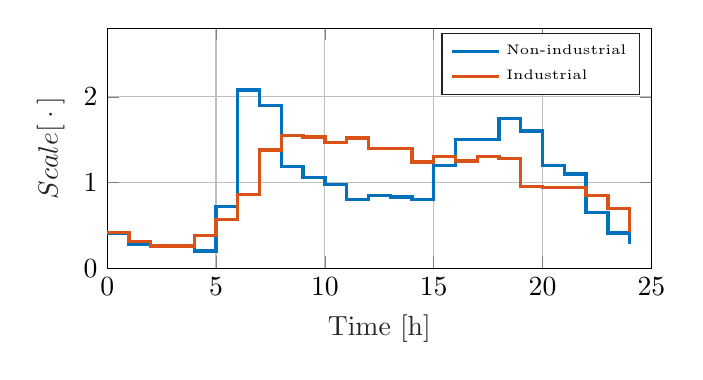
\begin{tikzpicture}

\begin{axis}[%
width=2.721in,
height=1.2in,
at={(0.758in,0.481in)},
scale only axis,
xmin=0,
xmax=25,
xlabel style={font=\color{white!15!black}},
xlabel={Time [h]},
ymin=0,
ymax=2.8,
ylabel style={font=\color{white!15!black}},
ylabel={$\text{Scale [}\cdot\text{]}$},
axis background/.style={fill=white},
%title style={font=\bfseries},
%title={Industrial/non-industrial water consumption pattern},
xmajorgrids,
ymajorgrids,
legend style={legend cell align=left, align=left, draw=white!13!black}
]
\addplot[const plot, color=mycolor1, line width=1.2pt] table[row sep=crcr] {%
0	0.41\\
1	0.280000000000001\\
2	0.25\\
3	0.260000000000002\\
4	0.199999999999999\\
5	0.719999999999999\\
6	2.08\\
7	1.9\\
8	1.19\\
9	1.06\\
10	0.98\\
11	0.800000000000001\\
12	0.850000000000001\\
13	0.829999999999998\\
14	0.800000000000001\\
15	1.2\\
16	1.5\\
18	1.75\\
19	1.6\\
20	1.2\\
21	1.1\\
22	0.649999999999999\\
23	0.41\\
24	0.280000000000001\\
};
\addlegendentry{\tiny Non-industrial}

\addplot[const plot, color=mycolor2, line width=1.2pt] table[row sep=crcr] {%
0	0.420000000000002\\
1	0.309999999999999\\
2	0.260000000000002\\
4	0.379999999999999\\
5	0.57\\
6	0.859999999999999\\
7	1.38\\
8	1.55\\
9	1.53\\
10	1.47\\
11	1.52\\
12	1.4\\
14	1.24\\
15	1.3\\
16	1.25\\
17	1.3\\
18	1.28\\
19	0.949999999999999\\
20	0.940000000000001\\
22	0.850000000000001\\
23	0.699999999999999\\
24	0.420000000000002\\
};
\addlegendentry{\tiny Industrial}

\end{axis}
\end{tikzpicture}%
\caption{Industrial and Non-industrial demand patterns in the EPANET simulation.}
\label{fig:demandpatterns_EPANET}
\end{figure}

It is worth noting that the industrial consumption profile in the VSV zone slightly differs from the industries in the rest of the network. However, since the VSV zone is not considered in the further simulation model, the demand pattern is not shown here. Furthermore, there are no consumers in the corresponding supply areas who have  significant effect on water consumption such that it influences the model calibration and simulation. 

\subsection{Pump stations and waterworks}
\label{pump_stations_andwaterworks}

As described in \secref{the_randers_water_supply_network}, there are several different pumping stations and waterworks in the network, supplying different zones. In general, there is a possibility in EPANET to simulate the cleaning process in the waterworks, including drilling, raw water and clean water treatment, however in the model the focus is on the correct distribution. Therefore all waterworks are simulated with using clean water reservoirs with. In the EPANET simulation, pumps in the waterworks pump the water out corresponding to the real pump curves. However, there is one exception, where the simulation of the pumping station is different. In the OMV water work, which is responsible for filling the tank(T1) in HBP pumping station in the HZ, the precise operation of the pumping station has not been taken into account. Instead, the control schedule of the pumps has been simulated as a positive demand node(negative according to the EPANET sign convention), just as in the network modelling, proposed in this report. The reason for this is that the controls turned out to be relatively complicated with frequency converters and simulation results of the pumping were not matching the real world scenarios. The advantage of this is that in one of the flow controlled pumping stations, the mass balance is controlled and furthermore the risk that the model does not simulate correctly is reduced. 
Apart from the OMV water work, all water works have been simulated with reservoirs which cannot be emptied by calculation. Water works and pumping stations, where the pumps are pressure controlled, are controlled by PRVs, as this is the typical way of controlling pressure controlled pumps in EPANET networks \cite{agency2016epanet}. Such an arrangement is shown in \figref{fig:PRV_EPANET} 

 %Waterworks in EPANET
\begin{figure}[H]
\centering
%\includegraphics[width=0.35\textwidth]{report/pictures/missingfigure}
\begin{tikzpicture}[scale=0.6,transform shape]

\begin{scope} [rotate around={0:(12,5.5)}, shift={(0.8,0)}]
\draw[thick,transform shape] (12,5.5) circle (0.5);
\draw[thick,transform shape] (12.5,5.5) -- (12,6);
\draw[thick,transform shape] (12.5,5.5) node (v1) {} -- (12,5);
\end{scope}

%man-valve
\begin{scope} [rotate ={-90}]
\node(n1) at (-5.25,16) {};
\draw[thick,transform shape](n1.center) -- ($(n1)-(0.5,0)$) --
($(n1)-(0,1)$) -- ($(n1)-(0.5,1)$) --  (n1.center);

\end{scope}

\draw [thick](15,5.5) -- (13.3,5.5);
\node at (15.5,6.2) {\large PRV};
\draw [thick](16,5.5) -- (17.5,5.5);
\draw [fill=cyan] [thick](9.1,5.7) -- (9.1,5.1) -- (10.9,5.1) -- (10.9,5.7);
\draw  [thick](9.1,6.1) -- (9.1,5.1) -- (10.9,5.1) -- (10.9,6.1);
\draw [thick](12.3,5.5) -- (10.9,5.5);
\end{tikzpicture} 
\caption{Water works modelled in EPANET, except OMV.}
\label{fig:PRV_EPANET}
\end{figure}

\vspace{-4mm}
It is important to note, however that with this arrangement in case of high demands in the network it is possible that water works and pumping stations deliver more flow than is actually possible. Therefore control rules have been incorporated in the models which prevents the pumping stations produce more flow than available in the real world. 

\section{Model calibration and validation}
\label{model_calibration_and_validation}

The simulation data has been validated by using pressure measurements on different fire hydrants in the network for several times in different years. When the model was made, the data was not completely up to date, as these pressure measurements were carried out in years before the EPANET modelling. The major uncertainty about this data is in the arrangement of the pipe network and the pumping stations, since it has been changed over the years and old facilities have been replaced. Although the data on which the model relies is uncertain and there might be variations in pressure, the validation of the model has been carried out according to these highly uncertain pressure measurements. 

\subsection{Pipe roughness}
\label{pipe_roughness}

In the model, all pipes are associated with tags, indicating dimensions, material and year information. With this information it is possible to estimate an average resistance, i.e. roughness of the pipes. 
During the validation process of the pipe resistances, it was chosen to consider an average roughness value, taking into account that the roughness should not be lower than a roughness of new pipes and at the same time, should not exceed a certain upper bound. Roughnesses were upscaled at places where the pressure was too high while downscaled where the pressure was certainly too low. Correct pressure data, however is an essential information for a more detailed and precise calibration, therefore high deviations are present in the system up to 5 meter heads. 

%Fire hydrants measurements
\begin{figure}[H]
\centering
\includegraphics[width=0.45\textwidth]{report/pictures/fire_hydrants}
%\begin{tikzpicture}[scale=0.6,transform shape]

\begin{scope} [rotate around={0:(12,5.5)}, shift={(0.8,0)}]
\draw[thick,transform shape] (12,5.5) circle (0.5);
\draw[thick,transform shape] (12.5,5.5) -- (12,6);
\draw[thick,transform shape] (12.5,5.5) node (v1) {} -- (12,5);
\end{scope}

%man-valve
\begin{scope} [rotate ={-90}]
\node(n1) at (-5.25,16) {};
\draw[thick,transform shape](n1.center) -- ($(n1)-(0.5,0)$) --
($(n1)-(0,1)$) -- ($(n1)-(0.5,1)$) --  (n1.center);

\end{scope}

\draw [thick](15,5.5) -- (13.3,5.5);
\node at (15.5,6.2) {\large PRV};
\draw [thick](16,5.5) -- (17.5,5.5);
\draw [fill=cyan] [thick](9.1,5.7) -- (9.1,5.1) -- (10.9,5.1) -- (10.9,5.7);
\draw  [thick](9.1,6.1) -- (9.1,5.1) -- (10.9,5.1) -- (10.9,6.1);
\draw [thick](12.3,5.5) -- (10.9,5.5);
\end{tikzpicture} 
\caption{Difference calculation between observed and calculated pressures on fire hydrants\cite{verdo_doc}.}
\label{fig:PRV_EPANET}
\end{figure}

\subsection{Grid balance and supply zones}
\label{grid_balance_supply_zones}

With the simulation model in EPANET it is possible to illustrate which pumping stations supply the different areas in the network. Simulations can be carried out for instance on supply areas in certain zones where more than one pumping station contributes to the consumption. The two zones, considered in this report are the HZ and LZ, in which the former is supplied by OMV and TBP and the latter is supplied by HBP and HSP where the tanks are placed on high elevation level. Consequently, as mentioned in \secref{waterworks_and_pumping_stations}, OMV and TBP are the waterworks and pumping stations which are responsible for filling the tanks in the HZ in HBP and HSP, respectively. \figref{fig:HSP_HBP_EPA} shows the distribution between the two pumping stations, HBP and HSP, in the high zone. 


\begin{figure}[H]
\centering
\begin{subfigure}{.49\textwidth}
\centering
  \includegraphics[width=0.75\textwidth]{report/pictures/HBP_HSP_distribution}
  \caption{HSP supply area, marked with red}
  \label{fig:HSP_HBP_EPA1}
\end{subfigure}
\begin{subfigure}{.49\textwidth}
\centering
  \includegraphics[width=0.75\textwidth]{report/pictures/HBP_HSP_distribution1}
  \caption{HBP supply area, marked with red}
  \label{fig:HSP_HBP_EPA2}
\end{subfigure}
\caption{Supply area by HSP(on the left) and supply area by HBP(on the right)(cite).}
\label{fig:HSP_HBP_EPA}
\end{figure}

The red areas in \figref{fig:HSP_HBP_EPA} indicate 80-100 percent of drinking water originating from one or the other pumping station. However, the other colours(primarily yellow and green) indicate that there is a mix of water from both stations. The result in the grid is according to the control goals, as one pumping station supplies half of the region and an other the other one. This is achieved by controlling the flow in HBP and the pressure in HSP. 

\section{Model preparation for data extraction}
\label{model_preparation_for_data_extraction}

\textbf{Discussion for supervisors for the meeting:}
\newline
\textcolor{blue}{Concerns: The two pumping stations in the high zone. The aim of these pumping stations is to distribute water to the grid in the high zone with the help of the watertanks. In EPANET the control is set such that the supply is nearly 50-50 percent. How to incorporate the effect of these into the model from which the data is extracted, since the pumping stations for control are considered to be the two stations in the low zone. Or is it even necessary if we do black box modelling? In the figure below the illustration is shown for help: }

%Fire hydrants measurements
\begin{figure}[H]
\centering
\includegraphics[width=1.2\textwidth]{report/pictures/supervisors}
%\begin{tikzpicture}[scale=0.6,transform shape]

\begin{scope} [rotate around={0:(12,5.5)}, shift={(0.8,0)}]
\draw[thick,transform shape] (12,5.5) circle (0.5);
\draw[thick,transform shape] (12.5,5.5) -- (12,6);
\draw[thick,transform shape] (12.5,5.5) node (v1) {} -- (12,5);
\end{scope}

%man-valve
\begin{scope} [rotate ={-90}]
\node(n1) at (-5.25,16) {};
\draw[thick,transform shape](n1.center) -- ($(n1)-(0.5,0)$) --
($(n1)-(0,1)$) -- ($(n1)-(0.5,1)$) --  (n1.center);

\end{scope}

\draw [thick](15,5.5) -- (13.3,5.5);
\node at (15.5,6.2) {\large PRV};
\draw [thick](16,5.5) -- (17.5,5.5);
\draw [fill=cyan] [thick](9.1,5.7) -- (9.1,5.1) -- (10.9,5.1) -- (10.9,5.7);
\draw  [thick](9.1,6.1) -- (9.1,5.1) -- (10.9,5.1) -- (10.9,6.1);
\draw [thick](12.3,5.5) -- (10.9,5.5);
\end{tikzpicture} 
\caption{Illustration for helping the discussion.}
\label{fig:PRV_EPANET}
\end{figure}

\textcolor{blue}{When data is extracted for system identification, it has to be considered that the pumping effort on P1 and P2 is not that high because the two pumping stations in the grid help in the high zone. }



















